\documentclass[11pt,a4paper]{article}

\usepackage[english,polish]{babel}
\usepackage[utf8]{inputenc}
\usepackage[T1]{fontenc}
\usepackage{lmodern}
\usepackage{indentfirst}
\usepackage{fullpage}
\usepackage{enumerate}
\usepackage{secdot}
\usepackage{verbatim}
\usepackage{listings}
\usepackage{graphicx}

\selectlanguage{polish}
\frenchspacing

% Zdefiniowanie autorów i~tytułu:
\author{Karol Dzitkowski}
\title{
	Aplikacje i usługi GIS\\
	\huge{Porównanie indeksów przestrzennych}\\
 	Dokumentacja wstępna
 } 	

\begin{document}
\maketitle
\newpage

% Wstawienie spisu tresci:
\tableofcontents
\newpage

%Treść:
\section{Cel projektu}
Porównanie różnego rodzaju indeksów przestrzennych i własnych pomysłów ze standardowo dostępnym indeksem przestrzennym w QGISie
(sprawdzenie wydajności wyszukiwania oraz odnajdywania najbliższych k punktów).
\section{Opis problemu}
Porównanie będzie polegało na przeprowadzeniu testów wydajności wyszukiwania, obliczania odległości, oraz innych operacji często
używanych w aplikacjach GIS, na dużym zbiorze danych. Porównywane będą indeksy przestrzenne oparte o:
\begin{enumerate}
	\item Brak indeksowania
	\item Functional Indexes np. lower(col1)
	\item GIN index
	\item B-Tree
	\item Geohashes
	\item Hilbert Curves
	\item GiST
	\item SP-GiST
\end{enumerate}
Wyniki przedstawiane będą w formie wykresów, a także w formie wygenerowanego raportu do pliku. Wyniki zostaną przeanalizowane i
po skończeniu projektu, zostanie utworzona dokumentacja opisująca wyniki i wyciągająca wnioski płynące z testów. Na tych samych danych
wejściowych zostanie przetestowana wydajność indeksowania dla systemu QGIS. Wyniki dla QGIS zostaną porównane do wyników wyżej opisanych 
testów w dokumentacji końcowej.
\section{Rozwiązanie}
\subsection{Program}
Rozwiązanie będzie oparte na technologii Microsoft $ASP.NET MVC4$ oraz będzie napisane głównie w języku $C\#$. Klient będzie zatem
systemem przeglądarkowym. Serwer oprogramowania będzie łączył się z bazą danych $PostgreSQL$ z wtyczką $PostGIS$ za pomocą biblioteki 
$Npgsql.dll$. Serwer w skutek zapytania od klienta, będzie odpalał odpowiednie procedury SQL i śledził czas ich wykonania, a następnie odsyłał wyniki. 
Program będzie umożliwiał porównywanie czasu wykonania różnych procedur/zapytań dla wszystkich, lub dwóch wybranych sposobów 
indeksowania. Czas wykonania w zależności od ilości danych do przetworzenia będzie prezentowany w formie wykresu. Wykresy 
generowane będą przy pomocy biblioteki $DotNet.Highcharts$ na licencji MIT. \\ 
Program klienta będzie składał się z jednego widoku: \\
\begin{figure}[ht!]
\centering
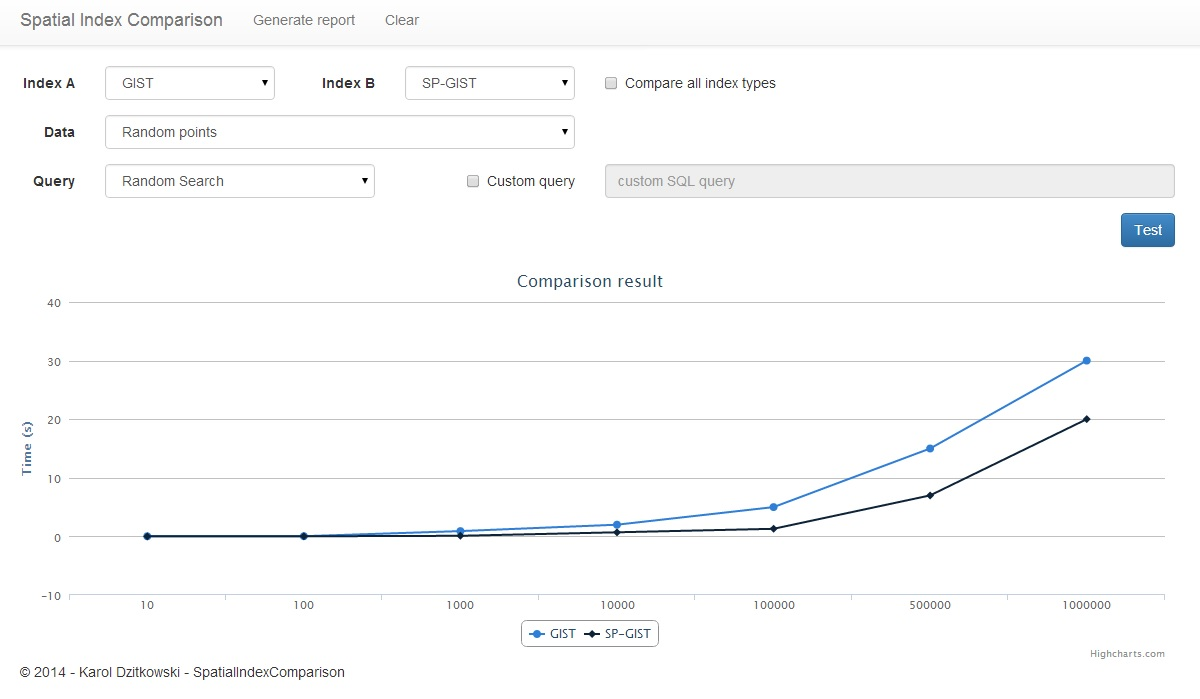
\includegraphics[width=\textwidth]{Program.jpg}
\caption{Widok programu}
\label{overflow}
\end{figure}
\\
\subsubsection{Opis programu}
W menu górnym widoczne będą dwa przyciski ,,Generate report'', który zapisywać będzie plik raportu w wybranym miejscu na dysku, oraz ,,Clear'' odświeżający opcje wyboru do stanu domyślnego. Poniżej menu znajdować się będą pola edycji umożliwiające wybór rodzajów indeksów do porównania, zapytania jakie ma być testowane oraz dane na których ma być uruchomione zapytanie. Możliwe również będzie wykonanie zapytania dla wszystkich rodzajów indeksów zaznaczając pole
,,Compare all index types''. Dodatkową funkcjonalnością będzie możliwość ręcznego wpisania zapytania (znając możliwą składnię) w pole tekstowe ,,custom SQL query''. Edycja tego pola będzie możliwa tylko po zaznaczeniu pola ,,Custom query''.
Naciśnięcie przycisku ,,Test'' spowoduje uruchomienie testów i odświeżenie diagramu. 
\subsection{Dane}
Testy przeprowadzane będą na zbiorach danych o różnej strukturze oraz różnej wielkości. Dane brane pod uwagę:
\begin{itemize}
	\item Punkty wygenerowane losowo
	\item Linie (pary punktów) wygenerowane losowo
	\item Prawdziwe dane dla Polski zaczerpnięte z GeoCommunity (www.geocomm.com) w formacie E00.
\end{itemize}
Dane w formacie E00 zostaną przekonwertowane programem e00pg i zaczytane do bazy PostgreSQL. Reszta danych zostanie 
wygenerowana za pomocą procedur SQL bezpośrednio na bazie.
\subsection{Testy}
Analiza oraz porównanie różnych sposobów indeksowania będzie opierała się na badaniu wpływu indeksowania na wydajność dla różnych
zestawów danych o różnych charakterystykach i właściwościach. np. dla punktów losowych, obejmujących całą przestrzeń wartości i dla punktów skupionych
w pewnych obszarach. Testowanie wyżej wymienionych metod indeksowania odbędzie się tylko i wyłącznie z użyciem programu, natomiast testy dla
wydajności indeksowania QGIS odbędą się przy użyciu programu QGIS z tymi samymi danymi zaimportowanymi z bazy PostgreSQL. Wyniki testów
zostaną przedstawione w dokumentacji końcowej w postaci tabeli oraz wykresów.

\section{Źródła}
\begin{itemize}
	\item $https://www.cs.purdue.edu/spgist/publications.xml$
	\item $http://drum.lib.umd.edu/bitstream/1903/1335/2/CS-TR-4556.pdf$
	\item $http://blog.notdot.net/2009/11/Damn-Cool-Algorithms-Spatial-indexing-with-Quadtrees-and-Hilbert-Curves$
	\item $http://informix-spatial-technology.blogspot.com/2012/01/comparison-on-b-tree-r-tree-quad-tree.html$
	\item $https://www.youtube.com/watch?v=53onZyrn8vA$
	\item $http://www.postgresql.org/docs/8.4/interactive/indexam.html$
	\item $https://www.pgcon.org/2011/schedule/attachments/197_pgcon-2011.pdf$
	\item $http://stackoverflow.com/questions/22602722/which-geo-implementation-to-use-for-millions-of-points$
	\item $http://e00pg.sourceforge.net/$
	\item $http://spatialnews.geocomm.com/education/tutorials/e00data/$
	\item $http://data.geocomm.com/catalog/PL/datalist.html$
\end{itemize}

\end{document}